\documentclass[11pt,twocolumn,twoside]{opticajnl}
%% Please use 11pt if submitting to AOP
% \documentclass[11pt,twocolumn,twoside]{opticajnl}

\journal{pr} % Choose journal (ao,jocn,josaa,josab,ol,optica,pr)

%See template introduciton for guidance on setting shortarticle option
\setboolean{shortarticle}{true}
% true = letter/tutorial
% false = research/review article
% (depending on journal)
\usepackage{lineno}
\usepackage[utf8]{inputenc}
\spanishdecimal{.}
\usepackage{amsmath}
\usepackage{caption}
\usepackage{subcaption}
\usepackage[spanish]{babel}
\usepackage{hyperref}
%\linenumbers


\title{

\vspace{-0.2cm} 

Trabajo práctico 1: Dinámica de sistemas acoplados}

\author[1]{Ignacio Lembo Ferrari}
\affil[1]{Instituto Balseiro - ignacio.lembo@ib.edu.ar 

\vspace{0.1cm}

13 de septiembre de 2023.}

\begin{abstract}
\textbf{Resumen: La dinámica con la que se forman estructuras en la arena está determinada por factores como el viento y la cantidad de arena disponible. En el presente trabajo, se emplearon diversos modelos de autómatas celulares para simular dichos factores con el objetivo de estudiar la morfología y la evolución temporal de ripples, dunas transversales y dunas barján. \\
Para cada estudio realizado, se detalló cada aspecto de la simulación así como también los parámetros y condiciones iniciales utilizadas. Dentro del estudio de los ripples, se caracterizó la influencia del viento en la longitud de onda característica de los mismos. Para las dunas barján, se estudió la dependencia funcional de la velocidad en función de la altura máxima de la duna.\\
Los resultados obtenidos para ripples y dunas como: escalas de tamaño, morfología, condiciones de formación y evolución temporal son compatibles con observaciones de campo y con simulaciones de trabajos anteriores.
}
\end{abstract}

\begin{document}

\maketitle

\section{Introducción \label{sec:intro}}

La morfología y dinámica de las estructuras de arena, como por ejemplo, las dunas, ha sido objeto de estudio principalmente de la geografía y la geología. No obstante, en los últimos años, ha cobrado gran interés entre los físicos consecuencia de la aparición de modelos que permiten describir propiedades de dichas estructuras. Debido a la dificultad para investigar sobre la dinámica de las dunas u otras estructuras, mediante mediciones de campo, se han propuesto modelos \cite{nishimori_formation_1993} \cite{katsuki_cellular_2011} que, junto con simulaciones numéricas permiten obtener información sobre la morfología y la evolución de las dunas.

La formación y evolución temporal de las estructuras de arena está determinada por la dirección e intensidad del viento y por la cantidad de arena disponible en el suelo \cite{bullard_wasson_2010}. A grandes rasgos, existen dos escalas de tamaño que dan lugar a estructuras de arenas significativamente diferentes. A escala pequeña, se forman los llamados ripples\footnote{En español: \textit{ondulita}, aunque es habitual llamarlos ripples} y a grandes escalas las dunas. 

Dentro de las dunas, existen dos tipos muy característicos: las dunas transversales y las dunas barján (ver Fig. \ref{fig:ej}). Las primeras, se forman debido a un flujo de viento unidireccional, perpendiculares a la dirección del mismo y en presencia de una gran cantidad de arena. Por otra parte, las dunas barján se forman cuando el flujo de viento es unidireccional pero la cantidad de arena es limitada.

\begin{figure}[H]
\centering
     \begin{subfigure}[b]{\linewidth}
        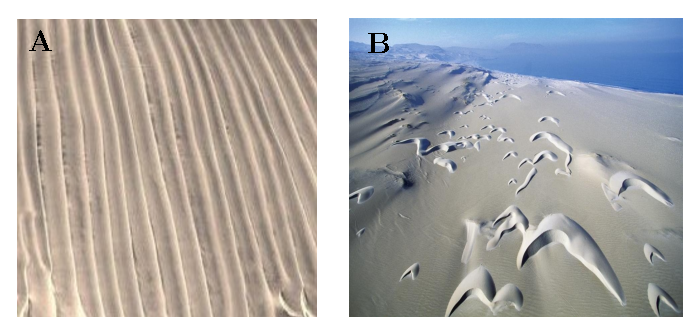
\includegraphics[width=\textwidth]{Figuras/dunas.eps}
         \label{fig:dunas}
     \end{subfigure}
\caption{\centering Imágenes típicas de dunas transversales (A) y dunas barján (B), extraídas de los trabajos de A. C. Sparavigna \cite{sparavigna_peruvian_nodate} y M. Talebpour \cite{mahdad_talebpour_numerical_2016} respectivamente.} 
\label{fig:ej}
\end{figure}

En este trabajo, se implementaron diversos modelos fenomenológicos simples que no profundizan en detalles de la dinámica de fluidos, con el objetivo de estudiar la formación de ripples, dunas transversales y dunas barján mediante simulaciones numéricas. En términos generales, dichos modelos consisten en un autómata celular bidimensional que tiene como procesos básicos el transporte (proceso en el cual se desplaza la arena debido al viento) y la relajación (proceso en el cual cae la arena debido a la gravedad en sentido contrario al gradiente de altura). A cada instante de tiempo de la simulación, ocurre el proceso de transporte para todas las celdas y luego, la relajación. 

\section{Modelos empleados}

El modelo consiste en un autómata celular bidimensional de dimensiones $L_x\times L_y$ con condiciones de borde periódicas. En esta grilla, cada celda representa una región donde la altura de arena es constante y es mucho mayor que el tamaño de un grano de arena. La variable $h(x,y,t)$ expresa la altura de arena en la celda $(x,y)$ a tiempo $t$. Se destaca que mientras que $x$, $y$, $t$ son variables discretas, $h(x,y,t)$ toma valores continuos. Como se mencionó anteriormente, la dinámica de evolución de este sistema sigue dos procesos básicos llamados transporte y relajación, los cuales se explican a continuación. 

\subsection{Transporte}

El transporte es el proceso en el cual los granos de arena son desplazados debido a la influencia del viento. Para este trabajo, se consideró el viento únicamente en la dirección $x$ positiva. A cada instante de tiempo, una cierta cantidad de masa $q$ es transportada en la dirección del viento de una celda $h(x,y)$ a otra celda $h(x + L, y)$. De esta manera, los cambios en las alturas de dichas celdas están dados por
\begin{equation}
    h(x,y) \rightarrow h(x,y) - q,
\end{equation}
y 
\begin{equation}
    h(x+L,y) \rightarrow h(x+L,y) + q.
\end{equation}

Se implementaron dos modelos para el transporte: el primero (modelo 1) extraído del trabajo de Katsuki A. et al. \cite{katsuki_cellular_2011} y el segundo (modelo 2) del trabajo de Nishimori-Ouchi \cite{nishimori_formation_1993}. 

\subsubsection{Modelo 1}

En este modelo, el desplazamiento $L$ en la dirección $x$ y la cantidad $q$ de arena que se transporta siguen las siguientes reglas
\begin{equation}
    L = L_0 + bh(x,y,t) - ch^2(x,y,t),
    \label{ec:Lmodelo1}
\end{equation}
\begin{equation}
    q \in [0,q_{max}],
\end{equation}
donde $q_{max} = 0.1$ se mantiene fijo y $L_0$, $b$, $c$ son parámetros a variar. Parte de este trabajo consiste en variar dichos parámetros y estudiar los cambios en la topografía de las estructuras de arena obtenidas. 

\subsubsection{Modelo 2}

El modelo 2 presenta dos variaciones con respecto al modelo 1. Primero, el desplazamiento está dado por 
\begin{equation}
    L = L_0 - b \tanh{ \biggr( \frac{dh}{dx}  \biggr) },
    \label{ec:Lmodelo2}
\end{equation}
donde $L_0$ y $b$ son parámetros a variar. Esto tiene en cuenta que el transporte $L$ de arena del lado de la duna con la que choca el viento es pequeño, mientras que en el lado de la duna donde no impacta el viento ocurre lo contrario. 
Además, la cantidad de arena $q$ que se desplaza está dada por 
\begin{equation}
q = q_0 + \Tilde{b} \tanh{ \biggr( \frac{dh}{dx} \biggr) },
\label{ec:qmodelo2}
\end{equation}
donde $q_0=1.0$ se mantuvo fijo en todo el trabajo y $\Tilde{b}$ es un parámetro a variar. Esto simula mayor cantidad de arena desplazada del lado de la duna con la que impacta el viento. 

Como se mencionó en la sección \ref{sec:intro}, la cantidad de arena disponible es un factor determinante en la formación de las dunas. Por lo tanto, para el estudio de las dunas transversales, el valor de cada celda $h(x,y,t)$ corresponde a la diferencia entre la altura de dicho punto y el valor promedio de toda la grilla. Con esto se simula un suministro abundante de arena, ya que para una dada celda siempre se puede extraer una cantidad $q$ de arena en el proceso de transporte. Por otra parte, para las dunas barján $h(x,y,t)$ indica la altura total de arena. En este caso, si la cantidad de arena a extraer $q$ de una celda es mayor a la cantidad de arena disponible en dicha celda $h(x,y,t)$, se extrae la cantidad $h(x,y,t)$. Con esto se simula el suministro limitado de arena. 

\subsection{Relajación}

Este proceso consiste en el desplazamiento de una cierta cantidad de arena $r$ en contra del gradiente de altura de arena, es decir, en dirección $-\nabla h(x,y,t)$. Más en detalle, dada una celda $(x,y)$, se busca la máxima diferencia de altura con sus primeras vecinas. Sea $(x',y')$ la celda que cumple esto, si la diferencia de altura $D = h(x,y) - h(x',y')$ es mayor a un valor $\Delta = 0.6$ (fijo para todos los estudios realizados) ocurre un desplazamiento de arena (relajación) según
\begin{equation}
    h(x,y) \rightarrow h(x,y) - r,
\end{equation}
y 
\begin{equation}
    h(x',y') \rightarrow h(x',y') + r.
\end{equation}
donde la cantidad $r$ es un valor aleatorio en el rango $[D/4, D/2]$, de manera que no se invierte el gradiente de altura que generó dicha relajación. 

\section{Formación de ripples}

Se estudió la formación de ripples aplicando el modelo 1 de transporte y se tomó $h(x,y,t)$ como la diferencia entre la altura del punto $(x,y)$ y el valor promedio de toda la grilla. Para ello, se partió de una condición inicial en una grilla de $500 \times 200$ donde $h(x,y,0)$ toma un valor aleatorio en el rango $[-0.5,0.5]$. Primero, se realizaron dos simulaciones para valores del parámetro $L_0=10$ y $L_0=30$ de la Ec. (\ref{ec:Lmodelo1}) dejando fijos $b=2.0$ y $c=0.01$. El resultado obtenido, para $1000$ pasos de tiempo, se muestra en la Fig. \ref{fig:ripples}.

\begin{figure}[H]
\centering
     \begin{subfigure}[b]{\linewidth}
        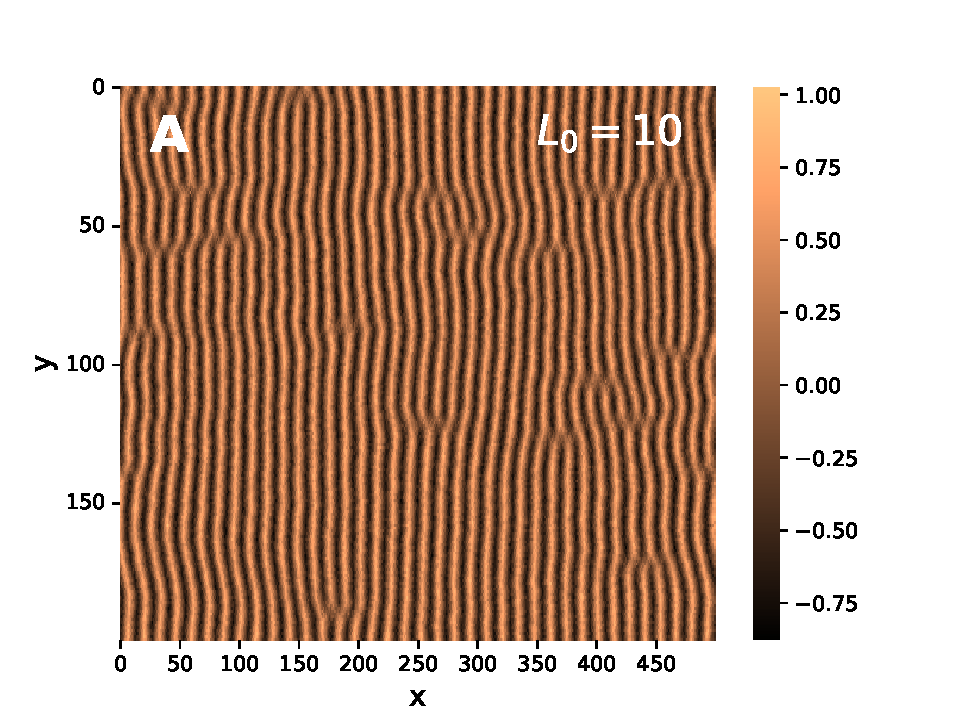
\includegraphics[width=\textwidth]{Figuras/ripple_L0=10.pdf}
         \label{fig:ripple_L0=10}
         \vspace{-1.5cm}
     \end{subfigure}
     \begin{subfigure}[b]{\linewidth}
         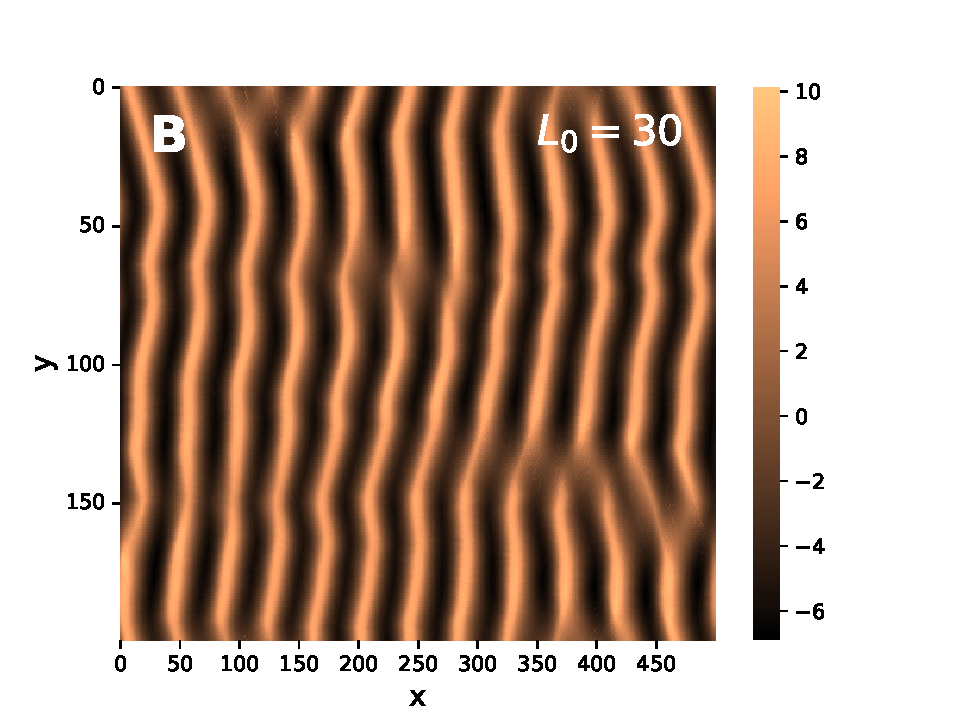
\includegraphics[width=\textwidth]{Figuras/ripple_L0=30.pdf}
         \label{fig:ripple_L0=30}
     \end{subfigure}
\caption{\centering Ripples obtenidos para una longitud de transporte $L = L_0 + bh(x,y,t) - ch^2(x,y,t)$ variando únicamente $L_0$  y partiendo de una condición inicial aleatoria $h(x,y,0) \in [-0.5,0.5]$. $h(x,y,t)$ representa la diferencia entre la altura de dicho punto y el valor promedio. La barra lateral muestra la escala de alturas. Parámetros: Grilla de $500 \times 200$, $1000$ pasos de tiempo, $b=2.0$ y $c=0.01$, $L_0 = 10$ (A) y $L_0 = 30$ (B).} 
\label{fig:ripples}
\end{figure}

Inspirado en los patrones periódicos obtenidos, se realizaron simulaciones variando únicamente el parámetro $L_0$ de la Ec. (\ref{ec:Lmodelo1}) con el objetivo de estudiar la influencia de dicho parámetro en la longitud de onda ($\lambda$) característica de los ripples. 

Para el análisis de la longitud de onda se aplicó la transformada de Fourier rápida al ripple obtenido para cada $L_0$ a $1000$ pasos de tiempo. A partir de los dos picos centrales de la transformada, se calculó la longitud de onda $\lambda$ para cada $L_0$ y se realizó una gráfica de $\lambda$ en función de $L_0$ como se muestra en la Fig. \ref{fig:lambdavsL}.

\begin{figure}[H]
\centering
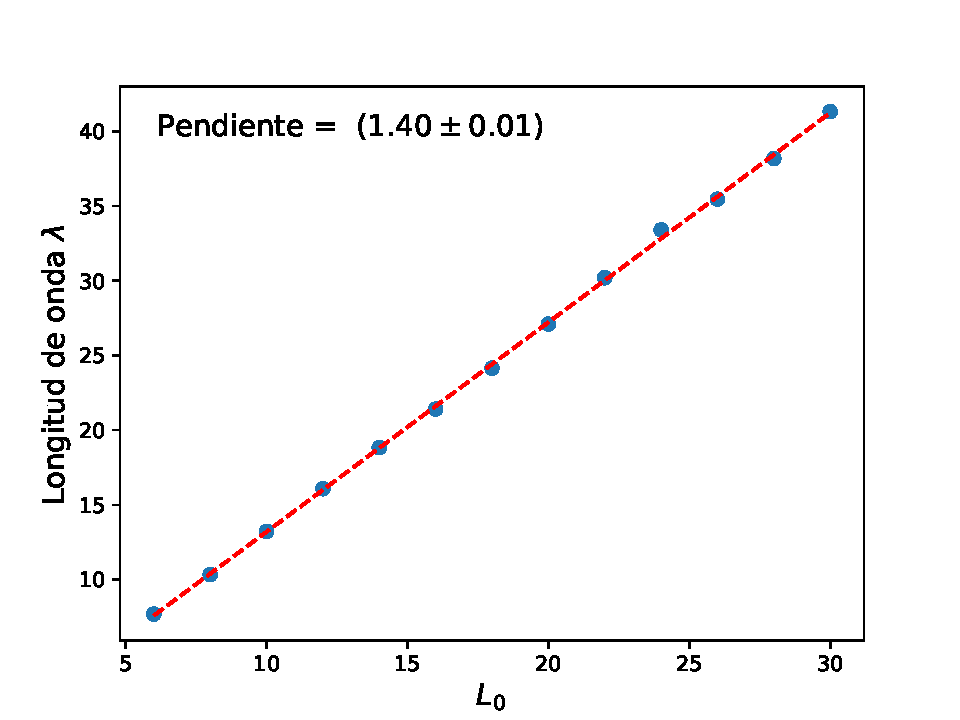
\includegraphics[width=\linewidth]{Figuras/fvsL0.pdf}
\caption{Longitud de onda $\lambda$ de los ripples en función del parámetro $L_0$. Se estudió la longitud de onda característica de ripples obtenidos para una longitud de transporte $L = L_0 + bh(x,y,t) - ch^2(x,y,t)$ variando únicamente el parámetro $L_0$. Parámetros: Grilla de $500 \times 200$, $1000$ pasos de tiempo, $b=2.0$ y $c=0.01$. Para valores de $L_0 < 6$ no se observó formación de ripples.}
\label{fig:lambdavsL}
\end{figure}

Como se puede ver en la Fig. \ref{fig:lambdavsL} se obtuvo una relación lineal entre la longitud de onda del ripple y el parámetro $L_0$, además se destaca que para valores de $L_0 < 6$ no se observó la formación de ripples. Todos estos resultados son consistentes con lo obtenido en trabajos anteriores para trabajos similares sobre ripples \cite{nishimori_formation_1993}.

\section{Dunas Transversales \label{sec:dunas_transversales}}

Para el estudio sobre la formación de dunas transversales se aplicó el modelo 2 de transporte y, debido a que la formación de dunas transversales se da cuando la cantidad de arena es limitada, $h(x,y,t)$ representa la diferencia entre la altura de dicho punto y el valor promedio de toda la grilla.

Se trabajó en una grilla de $500\times200$ partiendo de una cantidad aleatoria de arena $h(x,y,t) \in [4,6]$ para cada celda. Los parámetros utilizados en las Ecs. (\ref{ec:Lmodelo2}) y (\ref{ec:qmodelo2}) fueron: $L_0 =10$, $b=1.0$, $\Tilde{b} = 1.0$. La Fig. \ref{fig:dunas_transversales} muestra el resultado obtenido a $1000$ pasos de tiempo donde se ve que la morfología obtenida se corresponde con dunas transversales observadas en la naturaleza. 

\begin{figure}[H]
\centering
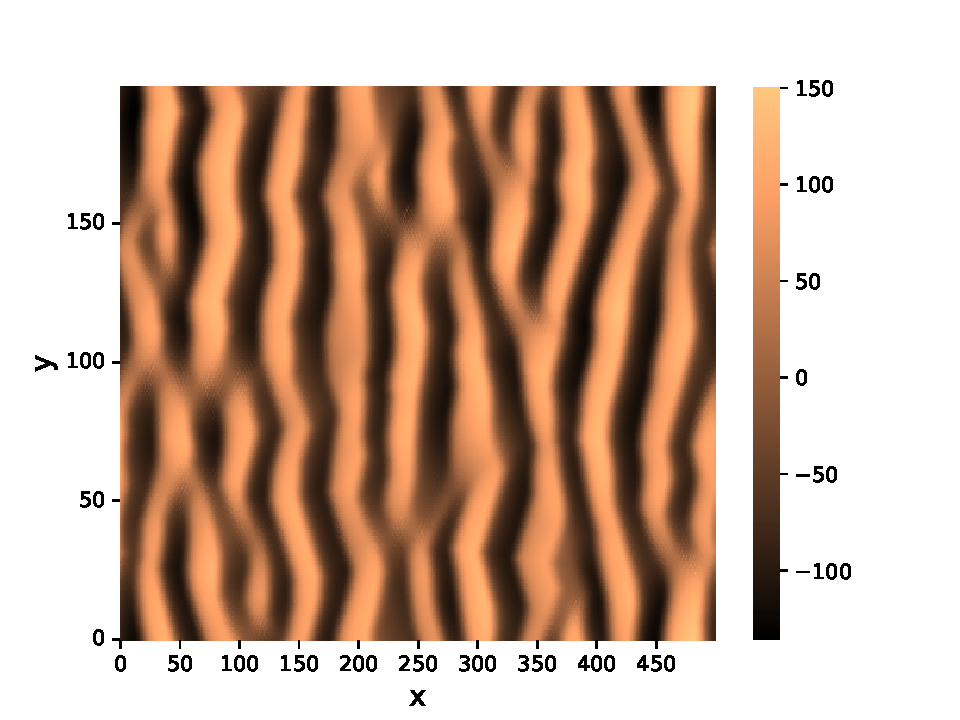
\includegraphics[width=\linewidth]{Figuras/dunas_transversales.pdf}
\caption{ \centering Dunas transversales obtenidas para una longitud de transporte $L = L_0 - b \tanh{  (dh/dx) }$ partiendo de una condición inicial aleatoria $h(x,y,0) \in [4,6]$. $h(x,y,t)$ representa la diferencia entre la altura de dicho punto y el valor promedio. La barra lateral muestra la escala de alturas. Parámetros: grilla de $500 \times 200$, $1000$ pasos de tiempo, $L_0 = 10$, $b=1.0$ y $\Tilde{b}=1.0$.}
\label{fig:dunas_transversales}
\end{figure}

La escala de tamaño de las dunas transversales es dos ordenes de magnitud mayor a la obtenida para los ripples, lo cual sustenta el hecho de que efectivamente son dunas. Este resultado permite afirmar que ambos modelos de transporte utilizados respetan la diferencia de escalas propias de los ripples y dunas. Entonces, se verifica que el modelo 1 modela bien la formación de ripples y el modelo 2 (considerando un suministro grande de arena) modela adecuadamente la formación de dunas transversales.

\section{Dunas barján}

Para el estudio sobre la formación de dunas barján se aplicó el modelo 2 de transporte. Se trabajó bajo las mismas condiciones iniciales y parámetros que en el estudio de las dunas transversales (sección \ref{sec:dunas_transversales}), pero considerando que la formación de dunas barján se da cuando la cantidad de arena es limitada. Por lo que $h(x,y,t)$ representa la altura total de arena en la  posición $(x,y)$. 

En la Fig. \ref{fig:muchos_barchanes} se muestra la grilla luego de $1000$ pasos de tiempo, resultado cualitativamente similar a la forma característica de las dunas barján y al resultado obtenido mediante simulaciones numéricas en trabajos anteriores \cite{nishimori_formation_1993}, donde se aplicaron modelos de transporte similares. Además, al igual que para las dunas transversales, la escala de tamaño obtenida es dos ordenes de magnitud mayor a la obtenida para los ripples, por lo que se concluye que se obtuvieron dunas. 

\begin{figure}[H]
\centering
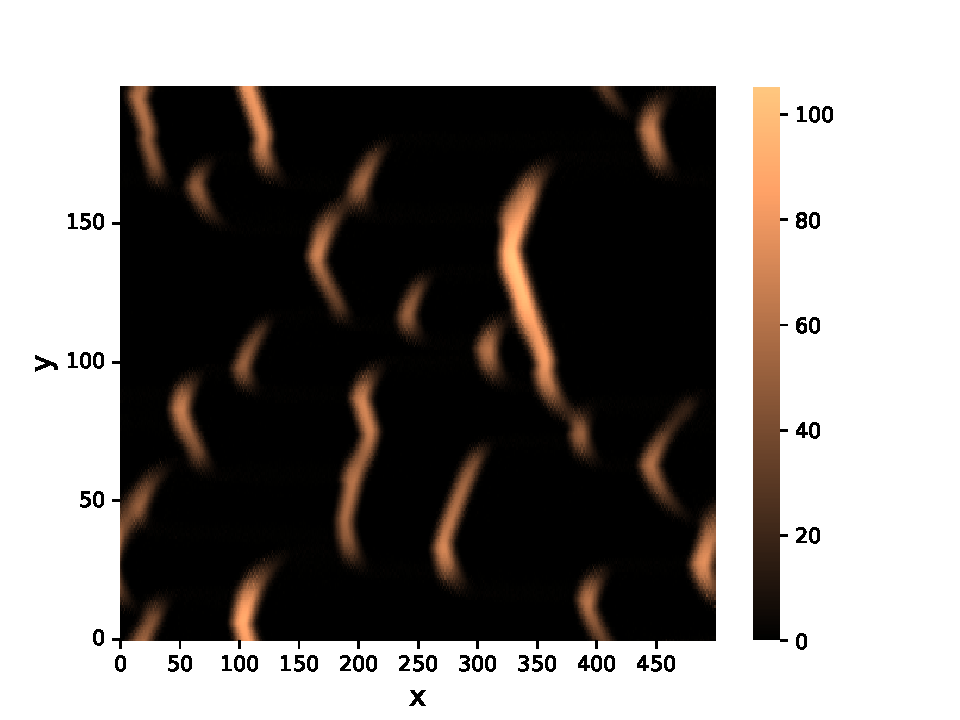
\includegraphics[width=\linewidth]{Figuras/muchos_barchanes.pdf}
\caption{\centering Dunas barján obtenidas para una longitud de transporte $L = L_0 - b \tanh{ (dh/dx) }$ partiendo de una condición inicial aleatoria $h(x,y,0) \in [4,6]$. $h(x,y,t)$ es la altura total de arena en la posición $(x,y)$. La barra lateral muestra la escala de alturas. Parámetros: grilla de $500 \times 200$, $1000$ pasos de tiempo, $L_0 = 10$, $b=1.0$ y $\Tilde{b}=1.0$.}
\label{fig:muchos_barchanes}
\end{figure}

Es importante destacar que las dunas barján obtenidas fueron simuladas bajo los mismos parámetros que las dunas transversales variando únicamente la condición del suministro de arena. Dado que esta es la condición que provoca, en la naturaleza, la formación de uno u otro tipo de duna \cite{bullard_wasson_2010}, se afirma que el modelo 2 de transporte reproduce exitosamente la formación de dunas en general y, bajo las condiciones necesarias, permite obtener buenos resultados para dunas transversales y barján. 

Para complementar los resultados, en el material suplementario \cite{link} se encuentra un video, a modo de ejemplo, sobre la formación de dunas transversales y barján obtenidas mediante las simulaciones realizadas. 

\subsection{Morfología de dunas barján\label{sec:morfologia}}

\begin{figure*}[t]
\centering
     \begin{subfigure}[b]{0.3\linewidth}
        \raggedleft
        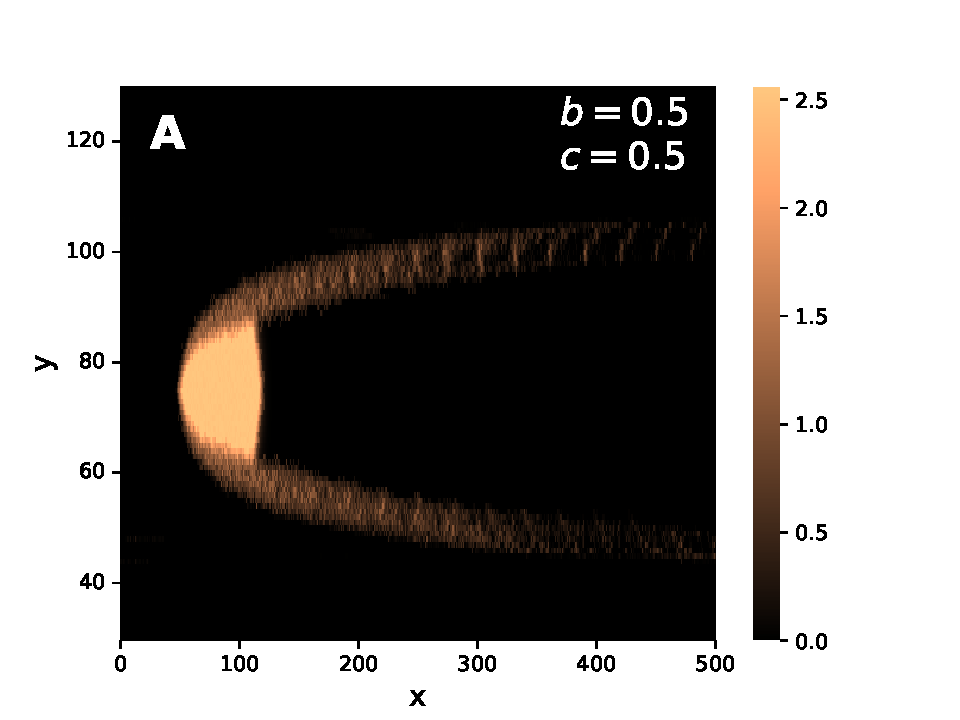
\includegraphics[width=1.1\textwidth]{Figuras/A.pdf}
         \label{fig:A}
     \end{subfigure}
     \begin{subfigure}[b]{0.3\linewidth}
        \centering
         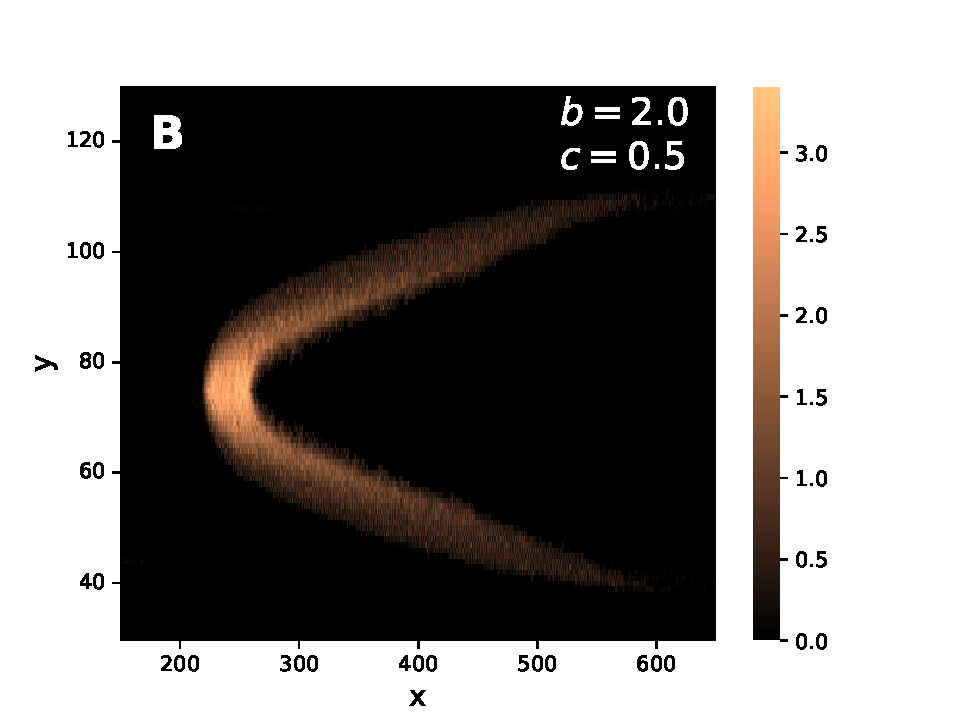
\includegraphics[width=1.1\textwidth]{Figuras/B.pdf}
         \label{fig:B}
     \end{subfigure}
    \begin{subfigure}[b]{0.3\linewidth}
        \raggedright
         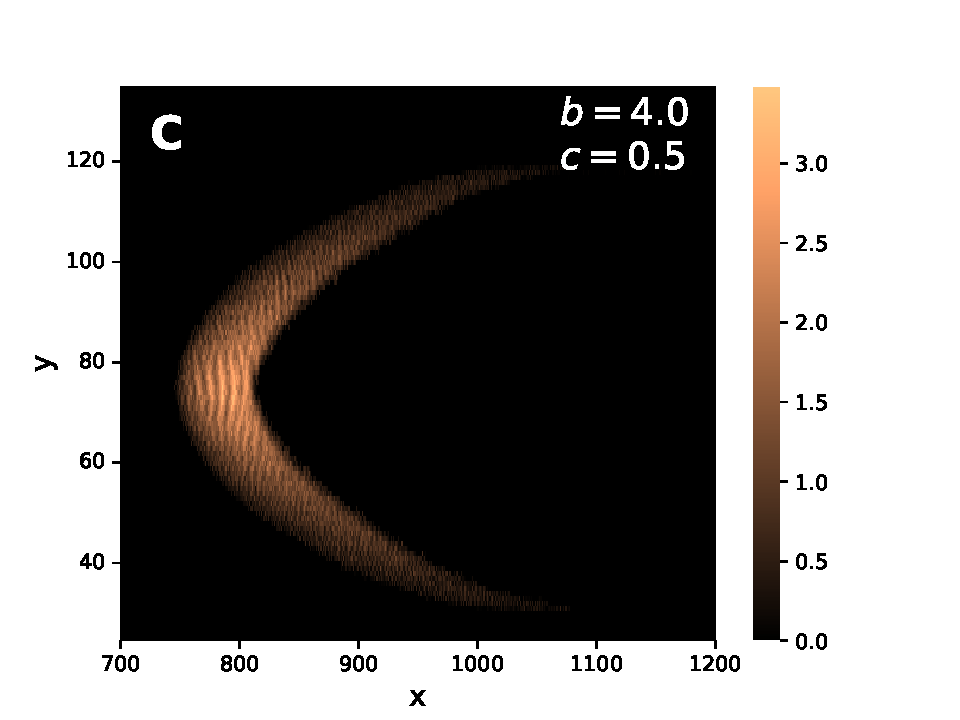
\includegraphics[width=1.1\textwidth]{Figuras/C.pdf}
         \label{fig:C}
     \end{subfigure}
          \begin{subfigure}[b]{0.3\linewidth}
          \raggedleft
         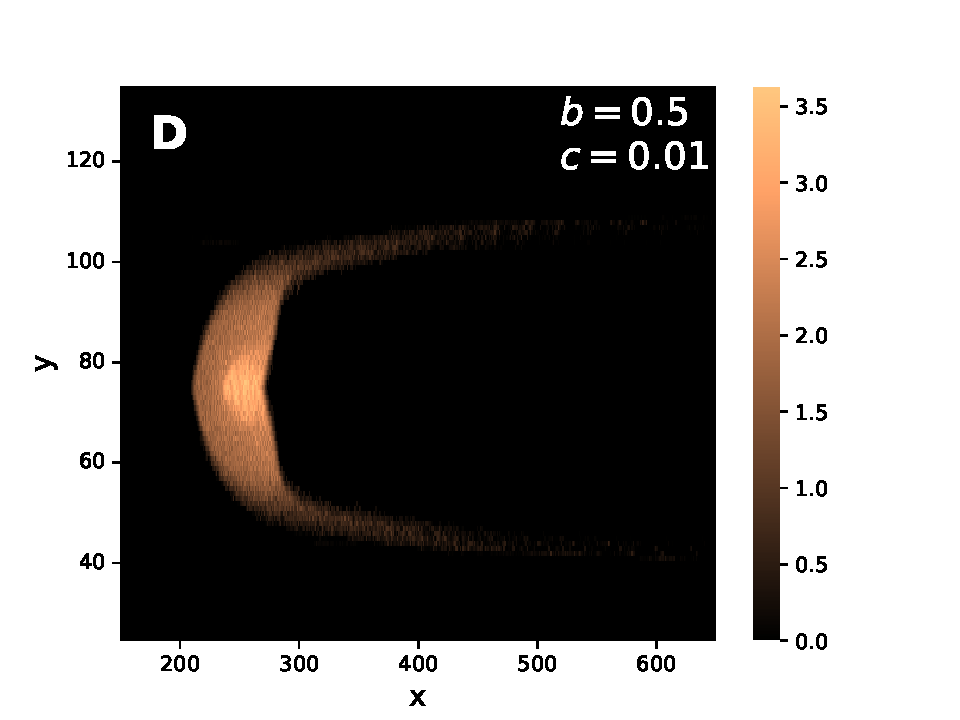
\includegraphics[width=1.1\textwidth]{Figuras/D.pdf}
         \label{fig:D}
     \end{subfigure}
          \begin{subfigure}[b]{0.3\linewidth}
          \centering
         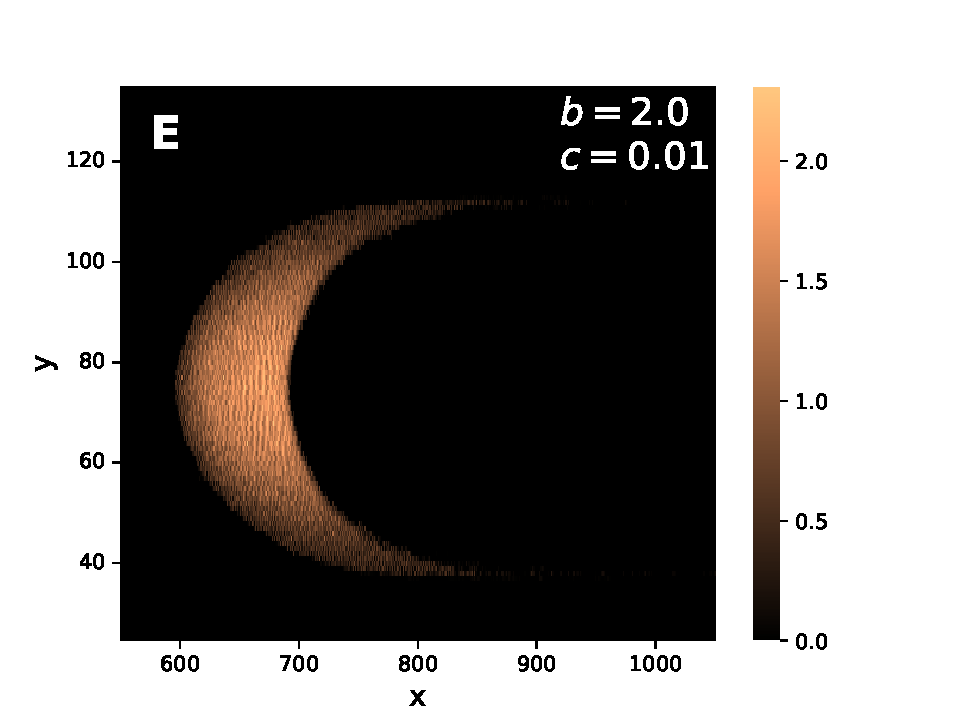
\includegraphics[width=1.1\textwidth]{Figuras/E.pdf}
         \label{fig:E}
     \end{subfigure}
    \begin{subfigure}[b]{0.3\linewidth}
        \raggedright
         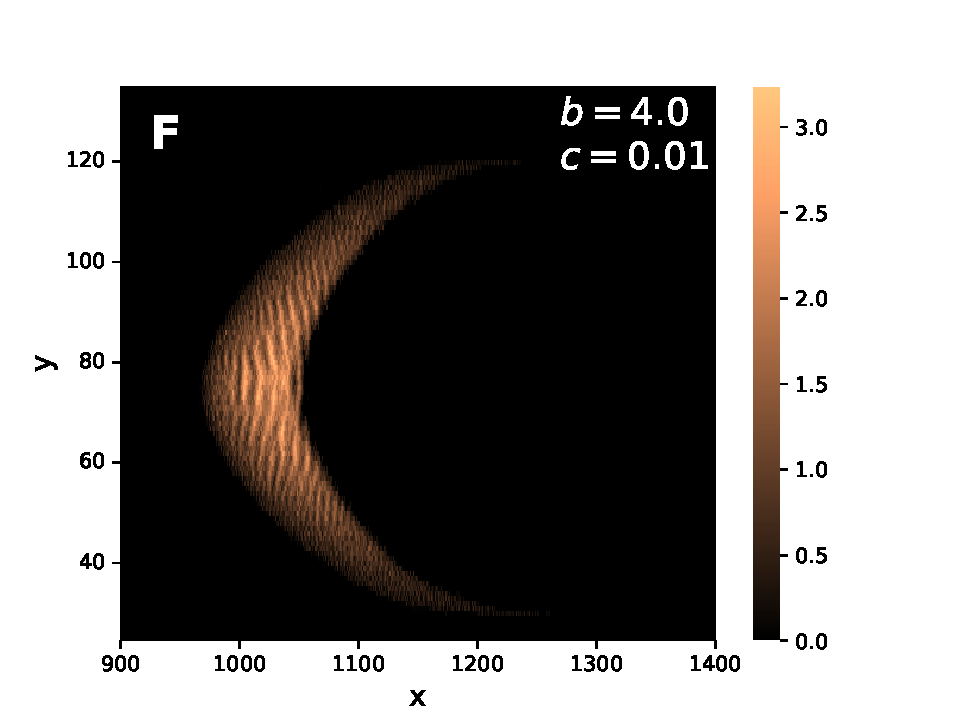
\includegraphics[width=1.1\textwidth]{Figuras/F.pdf}
         \label{fig:F}
     \end{subfigure}
\caption{\centering Estudio cualitativo de la morfología de las dunas barján para una longitud de transporte $L = L_0 + bh(x,y,t) - ch^2(x,y,t)$, partiendo de una condición inicial gaussiana . $h(x,y,t)$ es la altura total de arena en la posición $(x,y)$. La barra lateral muestra la escala de alturas. Parámetros: Grilla de $1500 \times 150$, $2500$ pasos de tiempo, $L_0 = 1.0$, de abajo hacia arriba $c=0.01,0.5$ y de izquierda a derecha $b=0.5,2.0,4.0$.}
\label{fig:morfología}
\end{figure*}

Tomando como referencia el trabajo de Katsuki A. et al. \cite{katsuki_cellular_2011}, y utilizando el modelo 1 de transporte, se realizó un estudio cualitativo de la morfología de las dunas barján en función de los parámetros de transporte $b$ y $c$ de la Ec. (\ref{ec:Lmodelo1}) dejando fijo $L_0=1.0$. No obstante, se implementó una variante de dicho modelo: para una cantidad de arena $h(x,y)$, si la altura de arena en posición $(x-\alpha L_0, y)$ cumple $h(x-\alpha L_0, y) > h(x,y)$ entonces no se produce transporte. El objetivo de esto es similar al del modelo 2 de transporte, simular el apantallamiento del viento debido a la presencia de dunas. Es decir, para arena que se encuentra del lado de la duna donde choca el viento se produce transporte, mientras que para la arena que se encuentra del otro lado no. El valor fenomenológico $\alpha$ se dejó fijo en $\alpha =50$.

Se trabajó en una grilla\footnote{La grilla es lo suficientemente larga en $x$ de modo que no afecten las condiciones de borde periódicas.} de $1500\times150$ y se tomó como condición inicial para cada simulación una gaussiana bidimensional dada por 
\begin{equation}
    h(x,y,0) = h_0 ~ \text{exp} \biggr( \frac{-(x-x_0)^2 - (y-y_0)^2}{2 \sigma^2} \biggr),
    \label{ec:gaussiana}
\end{equation}
con $\sigma^2=50$, $h_0 = 20$, $x_0=100$, $y_0=75$.  

En la Fig. \ref{fig:morfología} se presentan los resultados obtenidos para simulaciones de $5000$ pasos de tiempo para las 6 combinaciones de los parámetros $b=0.5,2.0,4.0$ y $c=0.01,0.5$ dejando $L_0=1.0$ fijo. Se observa que al aumentar $b$ la duna tiende a ser más ancha, es decir los extremos tienden a estar más abiertos, y al disminuir $c$ las dunas tienden a tener forma más redondeada lo que se asemeja más a observaciones de dunas barján en la naturaleza.  

En general, los resultados obtenidos en la Fig. \ref{fig:morfología} muestran como al variar los parámetros de la Ec. (\ref{ec:Lmodelo1}) se obtienen morfologías significativamente diferentes de las dunas. Además, se mostró que se puede desarrollar una única duna barján a partir de una pila de arena con forma gaussiana, lo cuál es de interés para diversos trabajos sobre la dinámica de interacción entre dunas barján \cite{katsuki_cellular_2011} \cite{katsuki_simulation_2011} \cite{katsuki_collision_2005}. 

\subsection{Evolución de las dunas barján}

Complementando al análisis de la sección anterior, se investigó la relación entre la movilidad de las dunas barján y la altura de la mismas aplicando la misma variante del modelo de transporte. Partiendo de una pila gaussiana de arena el estudio, consistió en medir para distintas alturas iniciales de la misma, la altura máxima y la posición del centro de masa de la duna formada en función del tiempo. 

Se dejaron fijos los parámetros de la Ec. (\ref{ec:Lmodelo1}) en $L_0=1.0$, $b=1.0$, $c=0.1$ y se tomó como condición inicial una pila gaussiana de arena dada por la Ec. (\ref{ec:gaussiana}) con $\sigma^2=50$, $x_0=100$, $y_0=75$ y con distintas alturas iniciales $h_0$ en el rango  $[1,30]$. Todas las simulaciones se realizaron con $2500$ pasos de tiempo. En el material suplementario \cite{link} se encuentra un vídeo típico, de la evolución de las dunas en las condiciones mencionadas. 

La Fig. \ref{fig:xvst} muestra la evolución temporal del centro de masa $x_{cm}$ y altura máxima $h$ para dunas barján con altura inicial $h_0=7,15,30$. 
\begin{figure}[H]
\centering
     \begin{subfigure}[b]{\linewidth}
        \centering
    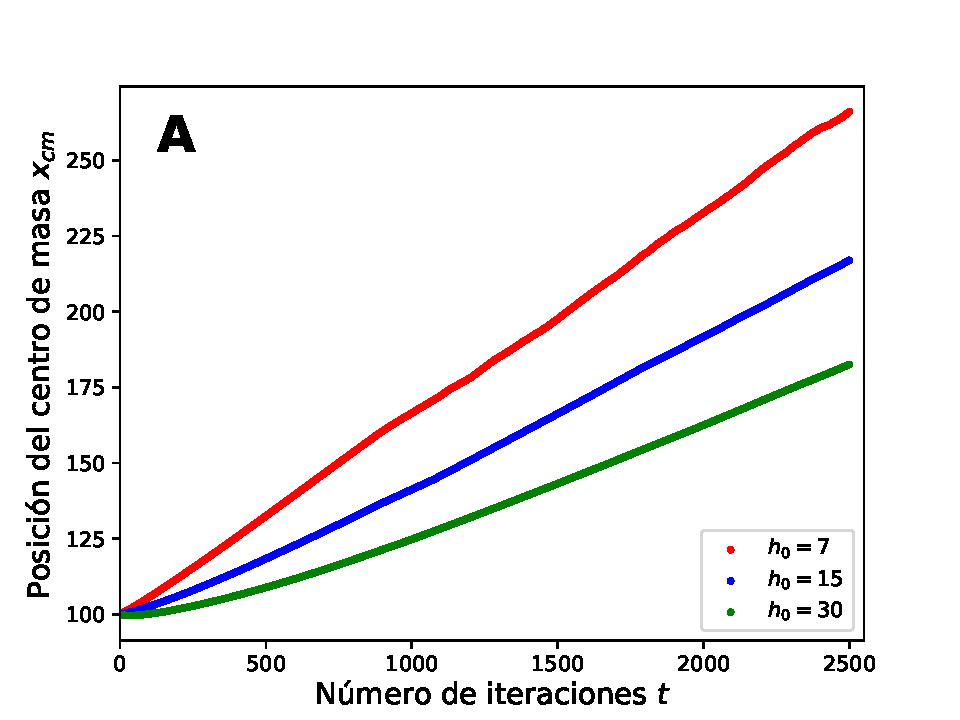
\includegraphics[width=0.8\textwidth]{Figuras/xvst.pdf}
         \label{fig:xcmvst}
     \end{subfigure}
     \begin{subfigure}[b]{\linewidth}
     \centering
     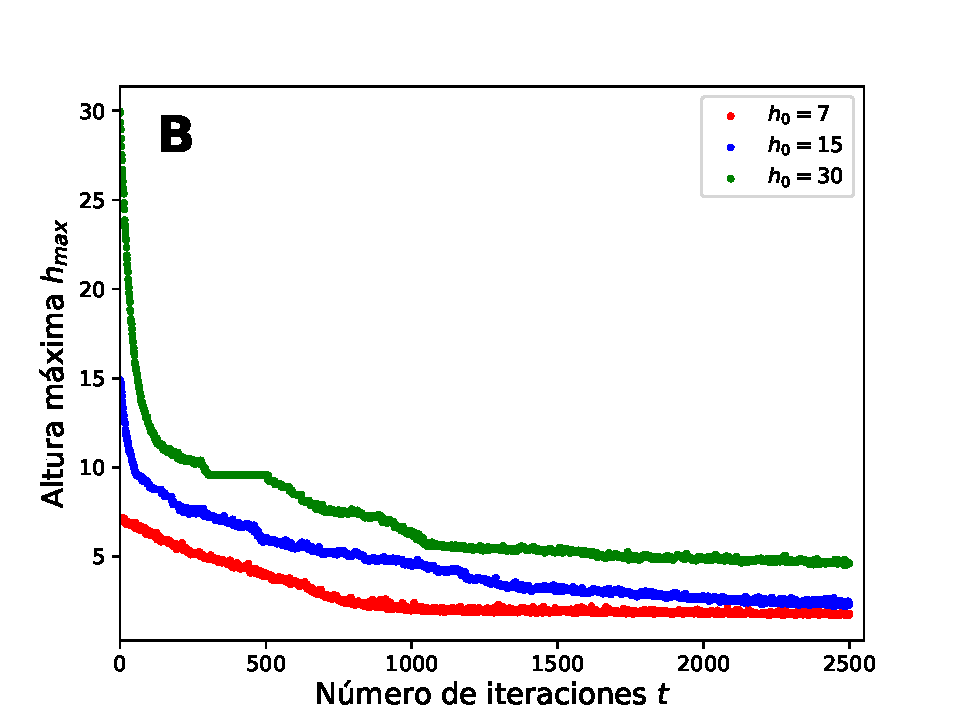
\includegraphics[width=0.8\textwidth]{Figuras/hvst.pdf}
         \label{fig:hvst}
     \end{subfigure}
\caption{\centering Evolución temporal del centro de masa $x_{cm}$ (A) y altura máxima $h$ (B) para dunas barján partiendo de una condición inicial gaussiana de altura $h_0=7$ (curva roja), $h_0=15$ (curva azul) y $h_0=30$ (curva verde).}
\label{fig:xvst}
\end{figure}

Se observa en la Fig. \ref{fig:xvst}, como la posición del centro de masa, luego de un transitorio, varía de forma lineal con el tiempo. Esto permite calcular la velocidad del centro de masa de cada duna $v_{cm,x}$ en la dirección $x$ a partir de un ajuste lineal de dicha curva. Además, se ve como la altura máxima de la duna decrece en función del tiempo hasta llegar a un valor aproximadamente estable para tiempos largos. 

En la Fig. \ref{fig:vvsh} se presenta la velocidad del centro de masa en función de la altura $h$ de la duna evaluados a $2500$ pasos de tiempo, valor de tiempo para el cual la altura máxima de la duna parece estabilizarse (ver Fig. \ref{fig:xvst}). Se ve como la velocidad del centro de masa decae en función de la altura, resultado compatible con mediciones de campo realizadas sobre dunas reales \cite{katsuki_cellular_2011}.

\begin{figure}[H]
\centering
    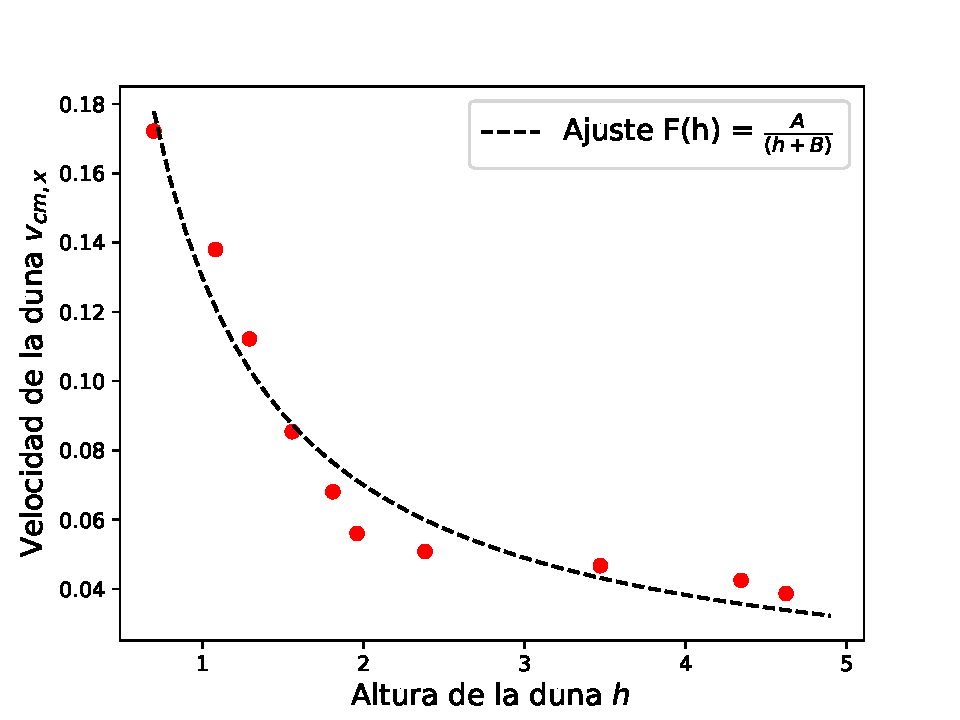
\includegraphics[width=0.8\linewidth]{Figuras/vvsh.pdf}
        \label{fig:vvsh}
\caption{\centering Relación morfológica entre la velocidad y la altura máxima de las dunas barján evaluadas a $2500$ pasos de tiempo para una longitud de transporte $L = 1.0 + 1.0~h(x,y,t) - 0.1~h^2(x,y,t)$, partiendo de una condición inicial gaussiana. $h(x,y,t)$ es la altura total de arena en la posición $(x,y)$. Se muestra en linea de trazo el ajuste según la función $v = A + \frac{B}{h+C}$. Parámetros: Grilla de $1500 \times 150$, $2500$ pasos de tiempo.}
\label{fig:vvsh}
\end{figure}

\vspace{0.7cm}

Para caracterizar la relación entre la velocidad y la altura de la duna desde un punto de vista cuantitativo, según Momiji et al. \cite{momiji_shape_2002} la velocidad de migración de la duna se puede ajustar según 
\begin{equation}
    v = A + \frac{B}{h+C},
    \label{ec:ajuste}
\end{equation} 
donde $A$, $B$ y $C$ son parámetros a ajustar y $h$ es la altura de la duna. Entonces, se ajustó con la Ec. (\ref{ec:ajuste}) la velocidad de la duna en función de su altura evaluados a $2500$ pasos de tiempo obteniendo $A=0.005$, $B=0.13$ y $C= 0.08$ como parámetros del ajuste (ver Fig. \ref{fig:vvsh}). Por lo tanto, se determina que la dependencia funcional de la velocidad con la altura ajusta bien por la Ec. (\ref{ec:ajuste}) considerando los tiempos de simulación implementados\footnote{En trabajos anteriores \cite{katsuki_cellular_2011} se han realizado simulaciones bajo el mismo modelo pero para tiempos de simulación de un orden de magnitud mayor. A estos tiempos la duna llega a una condición de estabilidad que permite obtener mejores resultados. No obstante, en este trabajo no se contaba con la capacidad de procesamiento para simular a tiempos tan largos.}. Lo cual aporta validez, en términos cuantitativos, al modelo utilizado para describir la evolución de las dunas barján. 


\section{Conclusiones}
\vspace{0.42cm}
En este trabajo, se emplearon diversos modelos de autómatas celulares para simular la dinámica del viento, con el objetivo de estudiar la morfología y dinámica de estructuras de arena como ripples y dunas. La principal diferencia entre dichas estructuras es la escala de tamaño que las caracteriza siendo los ripples de menor tamaño que las dunas. Dentro de las dunas, se analizaron las dunas transversales, que se caracterizan por formarse en presencia de un suministro de abundante arena y las dunas barján que, al contrario, se producen cuando el suministro de arena es escaso.

Un primer modelo \cite{katsuki_cellular_2011} permitió obtener satisfactoriamente los ripples en condiciones de suministro abundante de arena y se estudió la relación entre la fuerza del viento y la longitud de onda característica de los ripples. En particular, la relación entre la longitud de onda y el parámetro $L_0$ de la Ec. (\ref{ec:Lmodelo1}). Se obtuvo una relación lineal, resultado consistente con trabajos anteriores \cite{nishimori_formation_1993}.

Para estudiar las dunas se utilizó, un segundo modelo \cite{nishimori_formation_1993} que considera el apantallamiento del viento debido a la presencia de las dunas. Con este modelo, se realizaron simulaciones utilizando el mismo conjunto de parámetros y condiciones iniciales pero variando la condición del suministro de arena obteniendo dunas transversales con suministro de abundante arena y dunas barján con suministro de arena limitada. Este resultado le aporta gran validez al modelo utilizado ya que el suministro de arena es una de las principales diferencias entre los tipos de dunas estudiados. 

Por último, se implementó un tercer modelo \cite{katsuki_cellular_2011} para estudiar la morfología y evolución temporal de una duna barján partiendo de una pila de arena de forma gaussiana. Las formas de las dunas obtenidas a partir del estudio morfológico muestran como al variar los parámetros de la Ec. (\ref{ec:Lmodelo1}) se obtienen resultados significativamente diferentes en la forma de las dunas. 

Complementando esto último, se realizaron simulaciones para distintas alturas iniciales de la pila gaussiana y se evaluó, a mismo número de pasos de tiempo, la altura máxima de la duna en función de la velocidad. Los resultados obtenidos muestran que la velocidad del centro de masa decae en función de la altura máxima, resultado que concuerda con mediciones sobre dunas reales. Además, la dependencia funcional de la velocidad con la altura ajusta bien por la función $v_{cm,x}(h) = A + \frac{B}{h+C}$ propuesta en trabajos anteriores \cite{momiji_shape_2002}, concluyendo que el modelo utilizado es adecuado para describir cuantitativamente la movilidad de las dunas barján.

% Bibliography
\renewcommand*{\bibfont}{\normalsize}
\bibliography{FISCOM}

% Full bibliography added automatically for Optics Letters submissions; the following line will simply be ignored if submitting to other journals.
% Note that this extra page will not count against page length
\bibliographyfullrefs{FISCOM}

\centerline{\rule{0.95\linewidth}{0.6pt}}

\end{document}